\documentclass[10pt,a4paper]{article}
\usepackage[utf8]{inputenc}
\usepackage{fullpage}
\usepackage{graphicx}
\usepackage{fancyhdr}
\usepackage{occi}
\setlength{\headheight}{13pt}
\pagestyle{fancy}

\newcommand{\doccode}{XXXXX}

% default sans-serif
\renewcommand{\familydefault}{\sfdefault}

% no lines for headers and footers
\renewcommand{\headrulewidth}{0pt}
\renewcommand{\footrulewidth}{0pt}

% header
\fancyhf{}
\lhead{\doccode}
\rhead{\today}

% footer
\lfoot{occi-wg@ogf.org}
\rfoot{\thepage}

% paragraphs need some space...
\setlength{\parindent}{0pt}
\setlength{\parskip}{1ex plus 0.5ex minus 0.2ex}

% some space between header and text...
\headsep 13pt

\setcounter{secnumdepth}{4}

\begin{document}

% header on first page is different
\thispagestyle{empty}

\doccode \hfill Augusto Ciuffoletti, Univ. of Pisa\\ 
OCCI-WG \hfill Thijs Metsch, Intel Corp.\\
\rightline {Andy Edmonds, Zurich University of Applied Sciences}\\
\rightline {September 22, 2014}\\
\rightline {Updated: \today}

\vspace*{0.5in}

\begin{Large}
\textbf{Open Cloud Computing Interface - Notification Extension}
\end{Large}

\vspace*{0.5in}

\underline{Status of this Document}

This document provides information to the community regarding the
specification of the Open Cloud Computing Interface. Distribution is
unlimited.

\underline{Copyright Notice}

Copyright \copyright ~Open Grid Forum (2009-2011). All Rights Reserved.

\underline{Trademarks}

OCCI is a trademark of the Open Grid Forum.

\underline{Abstract}

This document, part of a document series, produced by the OCCI working
group within the Open Grid Forum (OGF), provides a high-level
definition of a Protocol and API. The document is based upon
previously gathered requirements and focuses on the scope of important
capabilities required to support modern service offerings.


\newpage
\tableofcontents
\newpage

\section{Introduction}
%!TEX root = nml-base.tex

\section{Introduction}%
\label{sec:introduction}

This document describes the base schema of the Network Markup Language (NML).
Section~\ref{sub:classes} defines the NML classes and their attributes and parameters.
Section~\ref{sub:relations} describes the relations defined between NML classes.

An NML network description can be expressed in XML\cite{xml}, and RDF/XML\cite{rdfxml} syntax.
Section~\ref{s:xmlschema} describes the XSD schema for the XML syntax.
Section~\ref{s:owlschema} describes the OWL 2 schema for the RDF/XML syntax.

These basic classes defined in this document may be extended, or sub-classed, 
to represent technology specific classes.

Section~\ref{s:examples} provides example use cases. This section is informative. 
Only sections~\ref{s:schema}, \ref{s:identifiers}, \ref{s:syntax}, and appendices \ref{s:xmlschema} and \ref{s:owlschema} are normative and considered 
part of the recommendation.

Appendix~\ref{s:g800terms} is informative and explains the relation between terms defined in this document and those defined in the ITU-T G.800 recommendation~\cite{g800}.

\subsection{Context}
\label{sec:context}

The Network Markup Language (NML) has been defined in the context of research and 
education networks to describe so-called hybrid network topologies. The NML is defined
as an abstract and generic model, so it can be applied for other network topologies as well.
See \cite{gfd.165} for an detailed overview including prior work.

\subsection{Scope}
\label{sec:scope}

The Network Markup Language is designed to create a functional description of 
multi-layer networks and multi-domain networks. An example of a multi-layered 
network can be a virtualised network, but also using different technologies. 
The multi-domain network descriptions can include aggregated or abstracted network topologies.
NML can not only describe a primarily static network topology, but also its potential capabilities (services) 
and its configuration.

NML is aimed at logical connection-oriented network topologies, more precisely topologies
where switching is performed on a label associated with a flow, such as a VLAN, wavelength or time slot. 
NML can also be used to describe physical networks or packet-oriented networks, 
although the current base schema does not contain classes or properties 
to explicitly deal with signal degradation, or complex routing tables.

NML only attempts to describe the data plane of a computer network, not the control 
plane. It does contain extension mechanism to easily tie it with network provisioning 
standards and with network monitoring standards.

Finally, this document omits a definition for the terms \emph{Network} or \emph{capacity}. 
This has been a conscious choice. The term \emph{Network} has become 
so widely used for so many diverse meanings that it is impossible to create a 
definition that everyone can agree on, while still expressing something useful.
See \emph{Topology} for the concept of a network domain and a \emph{Link} with multiple 
sources and sinks for the concept of a local area network.
The term \emph{capacity} is used by different technologies in such a different 
way (e.g.\ including or excluding the header and footer overhead) that it is better 
to let technology-specific extensions make an explicit definition.

\subsection{Notational Conventions}%
\label{sec:rfc2119}

The keywords “\MUST{}”, “\MUSTNOT{}”, “\REQUIRED{}”, “\SHALL{}”, “\SHALLNOT{}”, 
“\SHOULD{}”, “\SHOULDNOT{}”, “\RECOMMENDED{}”, “\MAY{}”,  and “\OPTIONAL{}” are 
to be interpreted as described in \cite{rfc2119}.
% except that the words do not appear in uppercase. 

This schema defines classes, attributes, relations, parameters and logic.
Objects are instances of classes, and the type of an object is a class.

Names of classes are capitalised and written in italics (e.g.\ the \emph{Node} class).
Names of relations are written in camel case and in italics (e.g.\ the \emph{hasNode} relation).
Names of identifiers and string literals are written in monspaces font (e.g. \texttt{Port\_X:in}).

Diagrams in this document follow the diagrammatic conventions of UML class diagrams.
\begin{itemize}
\item A subclass-superclass relationship is represented by a line with hollow triangle shape pointing to the superclass.
\item A whole-part relationship is represented by a line with a hollow diamond shape pointing to the whole (group).
\item A entity-relationship is represented by a line, optionally with numbers at each end indicating the cardinality of the relation. A named entity-relationship has a verb next to the line, and a filled triangle pointing to the object of the verb. (e.g. the entitity-relationship
\nmlrelation{BidirectionalPort}{*}{hasPort}{2}{Port} is named \emph{hasPort}, and each \emph{BidirectionalPort} is related to exactly 2 \emph{Port}s, and each \emph{Port} may be associated with zero, one or more \emph{BidirectionalPort}s.)
\end{itemize}



\section{Notational conventions}
All these parts and the information within are mandatory for
implementors (unless otherwise specified). The key words "MUST", "MUST
NOT", "REQUIRED", "SHALL", "SHALL NOT", "SHOULD", "SHOULD NOT",
"RECOMMENDED", "MAY", and "OPTIONAL" in this document are to be
interpreted as described in RFC 2119 \cite{rfc2119}.


\newcommand{\smx}{{\em notifier}}
\newcommand{\ntfl}{{\em notification}}

\section{Motivations}

It is often the case that an entity changes during its lifetime: for instance a {\em Compute} resource experiences a transient at the beginning of its lifetime during bootup \cite{occi:infrastructure}.

We want to give the provider the tools to allow the user to define entities such that their changes are observable.

We introduce an OCCI Extension that allows the user

\begin{itemize} 
\item to differentiate an OCCI resource that produces notifications, and 
\item to describe how such notifications are visible to other OCCI Resources.
\end{itemize}

\section{OCCI notification}

The way to define a property of an OCCI entity is to associate a mixin to it. So the straightforward way to assert that an entity is one whose changes are observable is by associating a mixin that is related with this property. We call this mixin \smx.

To define where a notification is directed the user instantiates a \ntfl\ link.

%\begin{figure}[!h]
%	{\centering \resizebox*{0.9\columnwidth}{!}{\rotatebox{270}
%	    {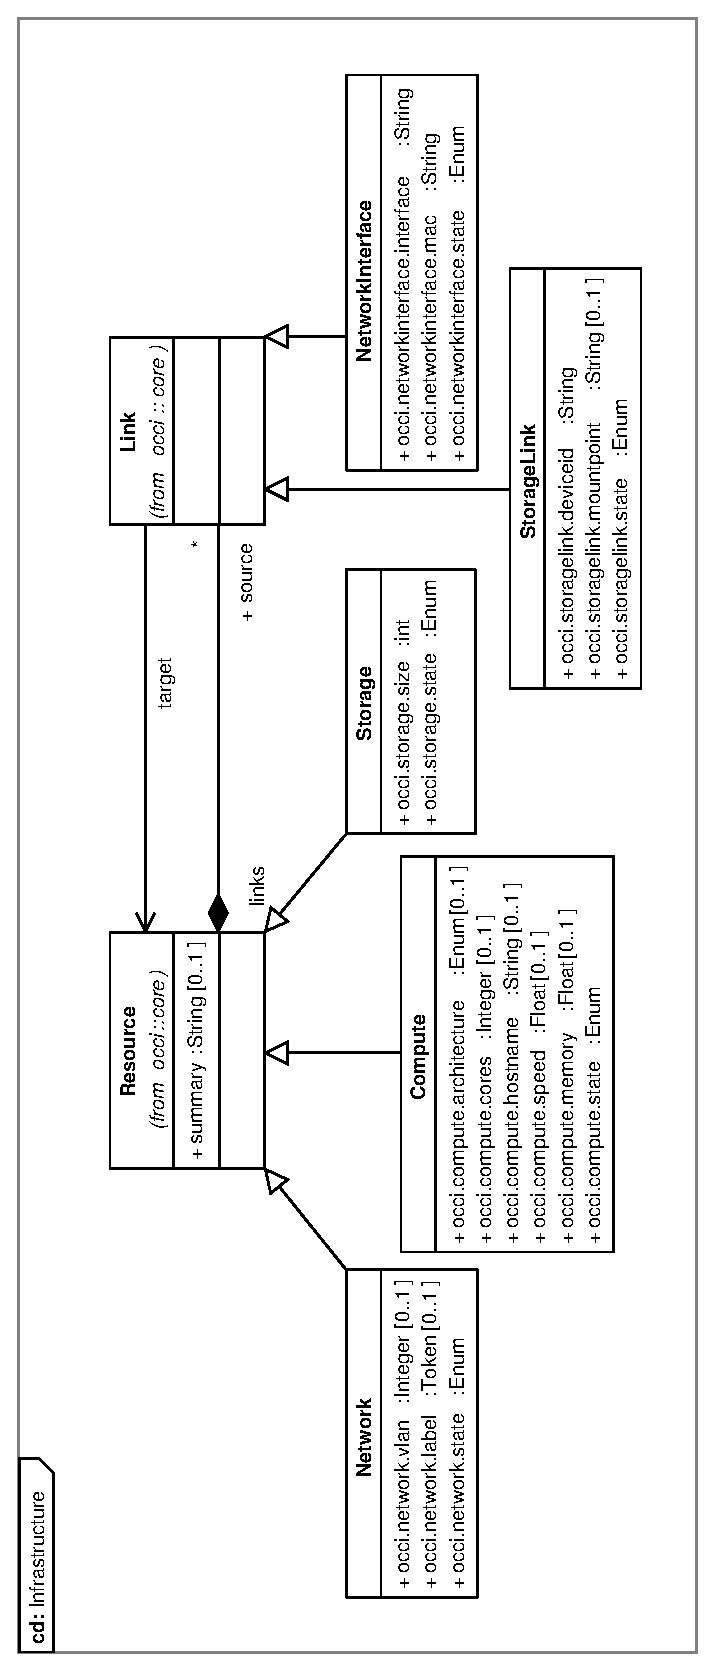
\includegraphics{figs/infrastructure_model.pdf}}} \par}
%	\caption{Overview Diagram of OCCI Infrastructure Types.}
%	\label{fig:infra_uml}
%\end{figure}


\subsection{The \smx\ mixin}

\mytablefloat{
	\label{tbl:smx}The immutable model attributes of the \smx\ mixin.
	The base URL {\bf http://schemas.ogf.org/occi} has been replaced with
	{\bf $<$schema$>$} in this table for a better reading experience. 
	} {
	\begin{tabular}{lllllll}
	\toprule
	Term & Scheme & Title & Attributes & Actions & Depends & Applies \\
	\colrule
	\smx &  $<$schema$>$/notification\# & \smx\ Mixin 
	& \{\} & \{\} & \{\} & $<$schema$>$/core\#Resource \\
	\botrule
	\end{tabular}
}

The {\em mixin} instance assigned to the \smx\ type is {\tt http://schemas.ogf.org/occi/notification\#notifier}, as in table \ref{tbl:smx}. The provider that supports the OCCI Notification extension MUST implement the \smx\ mixin for each provided entity kind.

There is no capability associated with the \smx\ mixin: it is a {\em tag}.

\subsection{The \ntfl\ link} 

\mytablefloat{
	\label{tbl:ntfl}The immutable model attributes of the \ntfl\ kind.
	The base URL {\bf http://schemas.ogf.org/occi} has been replaced with
	{\bf $<$schema$>$} in this table for a better readability experience. 
	} {
	\begin{tabular}{llllll}
	\toprule
	Term & Scheme & Title & Attributes & Actions & Parent \\
	\colrule
	\ntfl &  $<$schema$>$/notification\# & \ntfl\ Link
	& \{\} & \{\} & $<$schema$>$/core\#Link\\
	\botrule
	\end{tabular}
}

The {\em kind} instance assigned to the \ntfl\ type is {\tt http://schemas.ogf.org/occi/notification\#notification}, as in table \ref{tbl:ntfl}. The target of a \ntfl\ is a generic {\em Resource}, while the source MUST be associated with the \smx\ mixin. 

If the user requests the creation of a \ntfl\ whose source is not associated with a \smx\ mixin, the request MUST fail with an error.

If the user removes the \ntfl\ mixin associated with a {\em Resource}, all outgoing \ntfl\ links MUST be silently removed.

There is no capability associated with the \ntfl.

According with the core model \cite{occi:core}, the user is able to discover all \ntfl\ links that have their source in a given {\em Resource}.

According with the core model \cite{occi:core}, the removal of the source of an \ntfl\ link determines the removal of the link itself.

\section{Application notes and an example}

From the user perspective, the application of the \smx\ to a {\em Resource} corresponds to enabling the access to its state. This is significant mainly for {\em Resources} whose state changes in time.

The \smx\ mixin alone does not specify which changing aspect is in fact notified, and how: notably, not necessarily the attribute with {\sc state} id, if one exists. When needed, additional mixins are used to address specific events.

From the provider perspective the association of a \smx\ mixin is reflected in the implementation of the functionalities needed to observe and render the change. How this is implemented depends on the {\em Resources} that are targets of the \ntfl.

The way in which notifications are used falls ouside the scope of this document: as a general rule, they are for management purposes. Such aspects can be defined by the user with mixins associated with the \ntfl\ link, or in the {\em Resource} targeted by the \ntfl.

The notification extension is inappropriate to describe the planned and periodic measurement of operational parameters of a resource for monitoring purposes: the monitoring extension \cite{occi:monitoring} specifically addresses such aspects, and may be coordinated with notification.

The following example (see figure \ref{fig:example}) illustrates a use case where the capabilities of the involved entities are implicit in the {\em Kind} of the target resource.

\begin{figure}
\centering
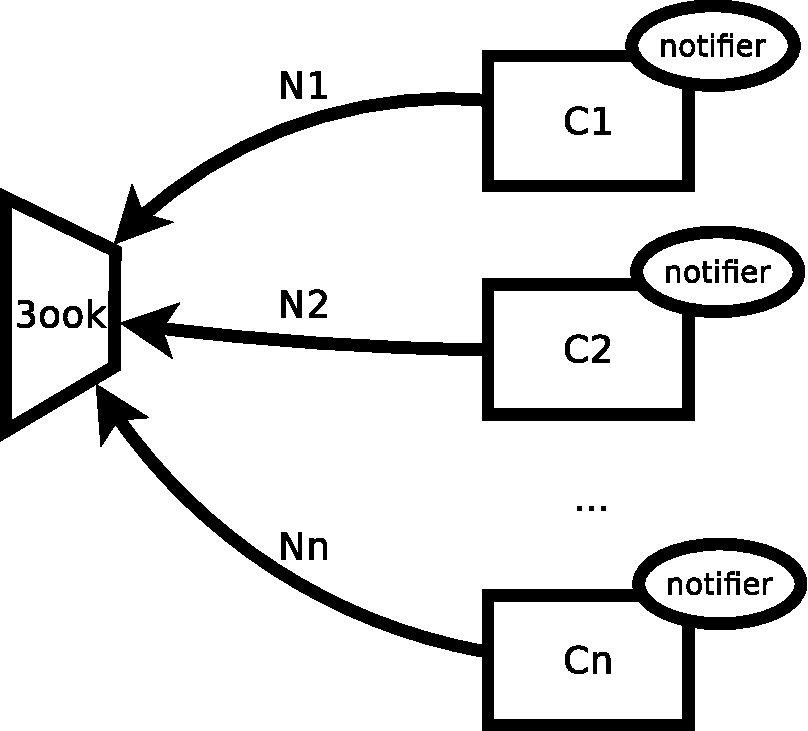
\includegraphics[width=0.4\textwidth]{figs/notificationExample.pdf}
\caption{Compute resources that notify their state to a control resource \label{fig:example}}
\end{figure}

\begin{quote}
A provider offers a Management Resource of {\em Kind} {\em 3-out-of-k}, that keeps in the {\em active} state three of the Compute resources from which it receives notifications.

The user that wants to take advantage of this service instantes a {\em 3-out-of-k} Resource $3ook$, and associates a \smx\ to each of the $k$ Compute resources $C_{1..k}$. For each of them a \ntfl\ link $N_i$ is instantiated that originates from $C_i$ and targets $3ook$.
\end{quote}

The schema is portable across any platform that offers the OCCI-infrastructure and OCCI-notification, and that provides a  {\em 3-out-of-k} {\em Kind}.

From the point of view of cloud management, the existence of a \smx\ entails the activation of a process that is able to detect and notify the occurrence of relevant events. The existence of a \ntfl\ corresponds to a kind of {\em subscribe} request: the occurrence of relevant events is notified to the target resource. 

The cloud management, knowing the type of resource that is the target of the notification, is able to optimize and configure the production of events and the notification protocol. However, such details are kept deliberatly hidden to the user, that has limited capabilities to configure the notifications service, bound to the existence of specialized mixins.

The API is therefore mostly opaque to the user: this is a feature of the notification service that is introduced to improve its useability, performance and robustness. Whenever the user needs better control on the monitoring process, for instance to perform custom management activities, the monitoring extension is preferable.

In figure \ref{fig:deploy} we give an idea of a possible deployment of a {\em 3ook} resource. The definition of the service attached to the resource is not relevant: all we need to know is that it controls resources based on notifications from the resources themselves, in a closed control loop. On the left side we see the virtual resources: the {\em 3-out-of-k} resource receives notifications in the form of {\sc xmpp} messages from the {\em notify processes} running on the Virtual Machine. The creation of this infrastructure is governed by the presence of \smx\ mixins and \ntfl. On the right there is the Cloud management architecture, that has control over the resources, in particular to process the input messages of the {\em 3ook} implementation (inside the container labelled {\em User Management}) and to control the state of the virtual machines (inside the container labelled {\em Resource Management}).

\begin{figure}
\centering
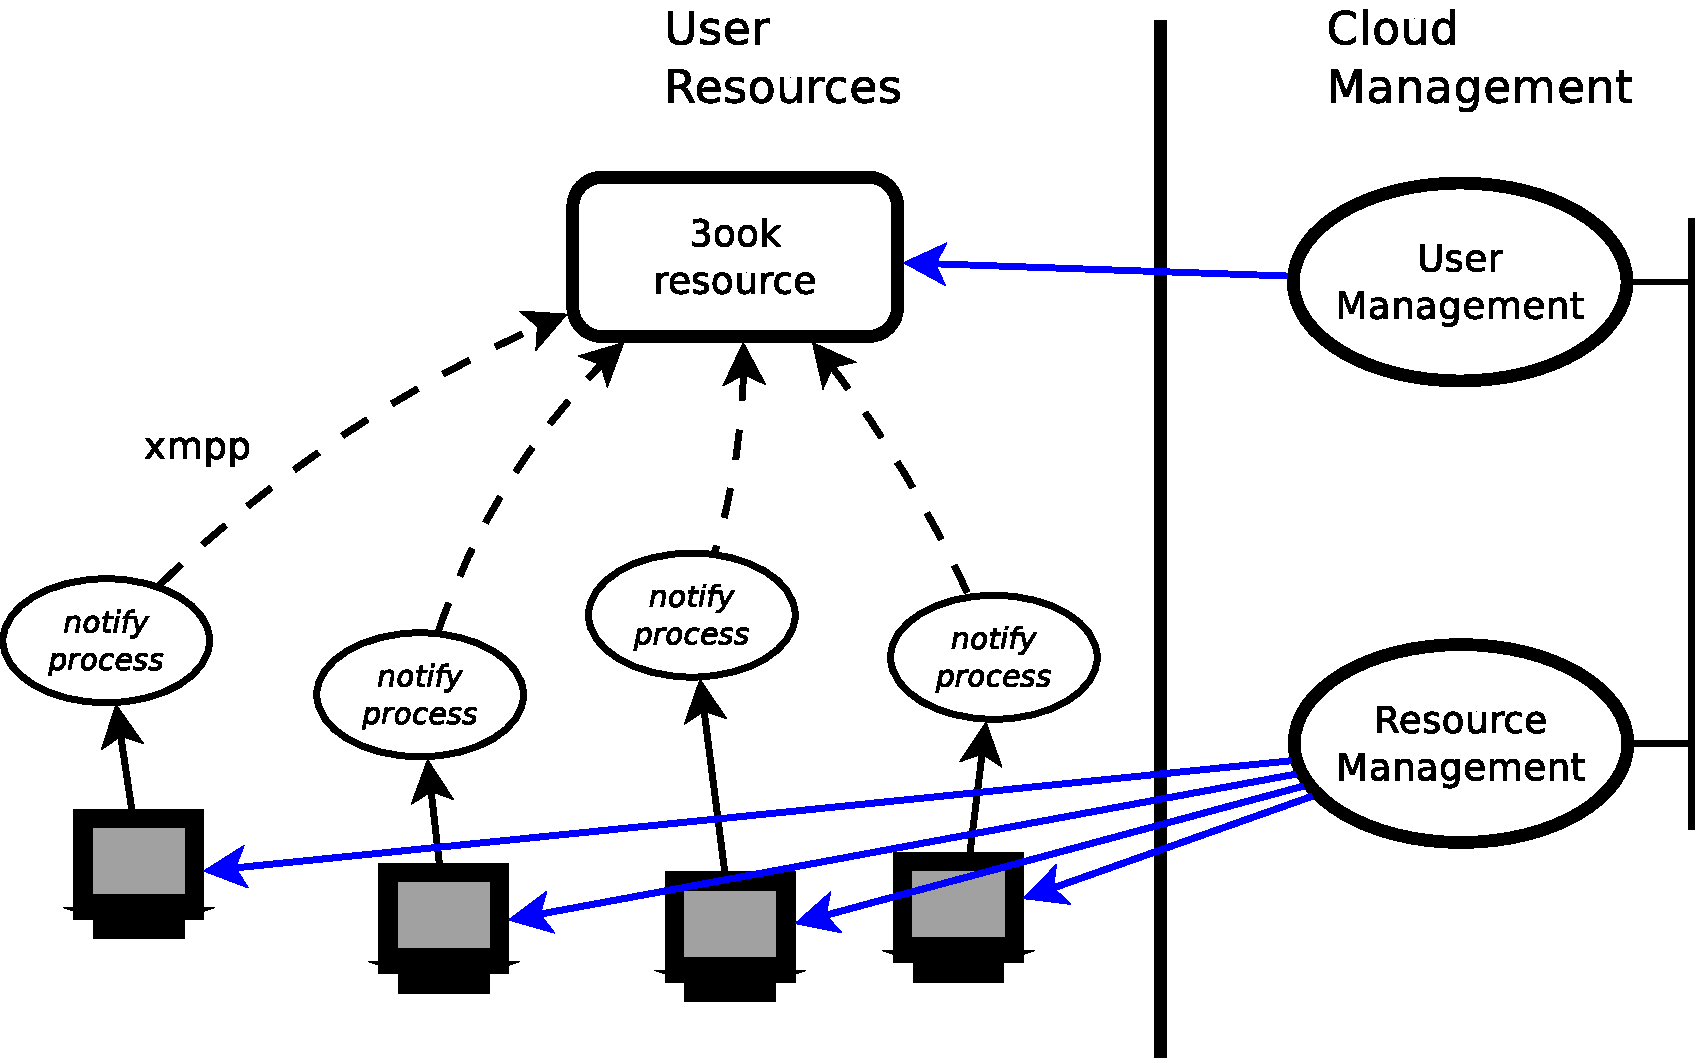
\includegraphics[width=0.6\textwidth]{figs/notificationDeploy.pdf}
\caption{Deploying a {\em 3ook} resource \label{fig:deploy}}
\end{figure}


Distinct providers may interoperate, if an agreement exists that allows cross-provider information transfer: for instance, one provides the  {\em 3-out-of-k} Resource and another the Compute resources.

\section{Security issues}
The OCCI Notification specification is an extension to the OCCI Core
and Model specification \cite{occi:core}; thus the same security
considerations as for the OCCI Core and Model specification apply
here.

\section{Glossary}
\label{sec:glossary}

\section{Glossary}
\label{s:glossary}

\begin{description}
\item[metric] a metric is a mathematical representation of a well defined aspect of a physical entity
\item[measurement] a measurement is the process of extracting a metric from a physical entity, and by extension also the result of such process. The measurement seldom corresponds exactly to the value of the metric.
\item[SLA] {\em ``An agreement defines a dynamically-established and dynamically
managed relationship between parties. The object of this
relationship is the delivery of a service by one of the parties within
the context of the agreement.''} from {\em SLA@SOI Glossary}
\item[Restful model] {\em ``REST is a coordinated set of architectural constraints that attempts to minimize latency and network communication, while at the same time maximizing
the independence and scalability of component implementations.''} \cite{fie02a}
\item[OCCI] {``\em The Open Cloud Computing Interface (OCCI) is a RESTful Protocol and API for all kinds of management tasks. OCCI was originally initiated to create a remote management API for IaaS model-based services, allowing for the development of interoperable tools for common tasks including deployment, autonomic scaling and monitoring''} \cite{occi:core}
\item[OCCI {\em Kind}] {\em''The Kind type represents the type identification mechanism for all Entity types present in the model''} \cite{occi:core}
\item[OCCI {\em \ln}] {\em''An instance of the Link type defines a base association between two Resource instances.''} \cite{occi:core}
\item[OCCI \mi] {\em''The Mixin type represent an extension mechanism, which allows new resource
capabilities to be added to resource instances both at creation-time and/or run-time.''} \cite{occi:core}
\item[OCCI \rs] {\em''A Resource is suitable to represent real world resources, e.g. virtual machines, networks, services, etc. through specialisation.''} \cite{occi:core}
\item[\sens] The \sens\ is a \rs\ that collects metrics from its input side, and delivers aggregated metrics from its output
\item[\coll] The \coll\ is a link that conveys metrics: it defines both the transport protocol and the conveyed metrics.
\end{description}

 
%\section{Contributors}
%
We would like to thank the following people who contributed to this
document:

\begin{tabular}{l|p{2in}|p{2in}}
Name & Affiliation & Contact \\
\hline
Michael Behrens & R2AD & behrens.cloud at r2ad.com \\
Mark Carlson & Toshiba & mark at carlson.net \\
Augusto Ciuffoletti & University of Pisa & augusto.ciuffoletti at gmail.com\\
Andy Edmonds & ICCLab, ZHAW & edmo at zhaw.ch \\
Sam Johnston & Google & samj at samj.net \\
Gary Mazzaferro & Independent &  garymazzaferro at gmail.com \\
Thijs Metsch & Intel & thijs.metsch at intel.com \\
Ralf Nyrén & Independent & ralf at nyren.net \\
Alexander Papaspyrou & Adesso & alexander at papaspyrou.name \\
Boris Parák & CESNET & parak at cesnet.cz \\
Alexis Richardson & Weaveworks & alexis.richardson at gmail.com \\
Shlomo Swidler & Orchestratus & shlomo.swidler at orchestratus.com \\
Florian Feldhaus & Independent & florian.feldhaus at gmail.com \\
Zden\v{e}k \v{S}ustr & CESNET & zdenek.sustr at cesnet.cz \\
\end{tabular}

Next to these individual contributions we value the contributions from
the OCCI working group.


\section{Intellectual Property Statement}
The OGF takes no position regarding the validity or scope of any
intellectual property or other rights that might be claimed to pertain
to the implementation or use of the technology described in this
document or the extent to which any license under such rights might or
might not be available; neither does it represent that it has made any
effort to identify any such rights. Copies of claims of rights made
available for publication and any assurances of licenses to be made
available, or the result of an attempt made to obtain a general
license or permission for the use of such proprietary rights by
implementers or users of this specification can be obtained from the
OGF Secretariat.

The OGF invites any interested party to bring to its attention any
copyrights, patents or patent applications, or other proprietary
rights which may cover technology that may be required to practice
this recommendation. Please address the information to the OGF
Executive Director.


\section{Disclaimer}
This document and the information contained herein is provided on an
``As Is'' basis and the OGF disclaims all warranties, express or
implied, including but not limited to any warranty that the use of the
information herein will not infringe any rights or any implied
warranties of merchantability or fitness for a particular purpose.


\section{Full Copyright Notice}
Copyright \copyright ~Open Grid Forum (2009-2011). All Rights Reserved.

This document and translations of it may be copied and furnished to
others, and derivative works that comment on or otherwise explain it
or assist in its implementation may be prepared, copied, published and
distributed, in whole or in part, without restriction of any kind,
provided that the above copyright notice and this paragraph are
included on all such copies and derivative works. However, this
document itself may not be modified in any way, such as by removing
the copyright notice or references to the OGF or other organizations,
except as needed for the purpose of developing Grid Recommendations in
which case the procedures for copyrights defined in the OGF Document
process must be followed, or as required to translate it into
languages other than English.

The limited permissions granted above are perpetual and will not be
revoked by the OGF or its successors or assignees.


\bibliographystyle{IEEEtran}
\bibliography{references}

\end{document}
